\phantomsection
\chapter[Random Walks and Turing Patterns]{Random Walks and Turing Patterns\chapsubhead{Noah Lee, Mert Inan, and Phillip Compeau}}
\label{chapter:turing}
\renewcommand{\chaptertitle}{Finding Motifs in Transcription Factor Networks}
\addcontentsline{cc}{chapter}{Chapter \thechapter} % Adds chapter number to table of contents


\FloatBarrier

\section{Turing and the Zebra’s Stripes}
\label{sec:introduction}
\phantomsection

Our story begins with an unlikely character: Alan Turing. If you have heard of Turing, then you might be surprised that he would appear in the first sentence of a course on biological modeling.

\begin{figure}[h]
\centering
\mySfFamily
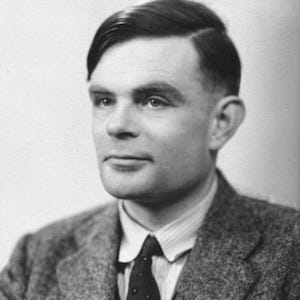
\includegraphics[width = 0.6\textwidth]{../assets/images/600px/alan_turing_npg_cc.jpg}
\caption{Alan Turing in 1951. © National Portrait Gallery, London.}
\label{fig:alan_turing_npg_cc}
\end{figure}

Turing was a genius cryptographer who helped break several German ciphers during World War II. But his most famous scientific contribution was a 1936 paper in which he introduced what has come to be known as a \textdef{Turing machine}{Turing machine}{FILL IN}. This hypothetical computer consists of an infinitely long tape of cells and a reader that can read one cell at a time. Each cell consists of only a single number, and the machine can move one cell at a time, reading and rewriting cells according to a finite collection of internal rules.

Turing's major insight was that this simple machine is nevertheless powerful. Nearly a century after his work, any task that can be performed by a computer --- even the world's most largest supercomputer --- could be implemented by a Turing machine, which Joseph Weizenbaum called nothing more than "pebbles on toilet paper".

Two years before his untimely demise in 1954, Turing published his only paper on biochemistry, which addressed the question: “Why do zebras have stripes?”

Turing was not asking why zebras have \textit{evolved} to have stripes --- this question was unsolved in Turing's time, and recent research has indicated that the stripes may be helpful in warding off flies. Rather, Turing was interested in what mechanism could produce the stripes that we see on a zebra's coat. And he reasoned that just as a simple machine can emulate a computer, some limited set of molecular "rules" could cause stripes to appear on a zebra's coat.

In this prologue, we will introduce a particle simulation model based on Turing's ideas. We will be amazed that a system built on very simple rules and even \textit{randomness} can nevertheless produce seemingly complex emergent behavior. And we will explore how this model can be tweaked to provide a hypothesis for the source of not just the zebra's stripes but also the leopard's spots.

\FloatBarrier
\phantomsection
\subsection{Life is random}

Everything in the universe ultimately depends on the interaction of tiny particles. Yet this fundamental truth is difficult to process when our experience of existence is guided by "macro" phenomena.

You may feel like a single, coherent being, but you are just a skin-covered bag of trillions of cells that act largely independently. Over half of these cells aren't even yours! They correspond to bacteria that make up a couple of kilograms of your mass. What makes the whole affair even crueler is that your cellular symphony depends on the \textit{random} movement of particles.

Throughout this course, we will see that just because a system is driven by randomness and simple rules does not mean that it cannot have emergent behavior that is complex and elegant. Just like you.

\FloatBarrier
\phantomsection
\subsection{The wanderlust of a randomly walking particle}

Cells are full of \textdef{proteins}{proteins}{FILL IN}, complex macromolecules that perform nearly every cellular function. If a protein could move in a straight line, then it would move at 20 kph or faster, but the cytoplasm that fills the cell is so densely packed with water molecules that the protein ping-pongs off them, frequently changing direction.

We will model the movements of a cellular particle such as a protein by a \textdef{random walk}{random walk}{FILL IN} in a two-dimensional plane. At each step, the particle moves a single unit of distance in a randomly chosen direction. The video below shows a randomly walking particle taking 1000 steps.

\texttt{NEED FIGURE HERE -- TO REPLACE VIDEO}\\

The distance that the particle wanders from its starting point may surprise you. And yet perhaps this particle is just an outlier, and the typical particle would be much more of a homebody.

\FloatBarrier
\phantomsection
\subsection{From one particle to many}

If we animate the action of many independent particles following random walks, then although some particles hug the starting point and some wind up far away, most particles steadily drift outward. The following video shows a simulation of 200 randomly walking particles.

\texttt{NEED FIGURE HERE -- TO REPLACE VIDEO}\\

In fact, although the movements of a single particle are random, we can draw conclusions about the \textit{average-case} behavior of many particles can be predicted, as the following theorem indicates.

\textdef{Random Walk Theorem}{Random Walk Theorem}{FILL IN} After \textvar{n} steps of unit length in a random walk, a particle will on average find itself a distance of approximately $\sqrt{n}$ from its origin.

\begin{note}[%
If you love mathematics and are interested in seeing a proof of this theorem, check out https://biologicalmodeling.org/assets/tex/random_walk_theorem.pdf 
]\end{note}

Our experience of the world confirms the Random Walk Theorem's statement that randomly walking particles tend to drift away from their starting point. We understand, for example, that an infected COVID-19 patient can infect many others in an enclosed space in a short time frame. To take a less macabre example, we also know that when a cake is baking in the oven at home, we will not need to wait long for wonderful smells to waft outward from the kitchen.

If you are interested in seeing how to build the random walk simulation shown in the video above, then please visit the following software tutorial. This tutorial uses \textdef{CellBlender}{CellBlender}{FILL IN}, an add-on to the popular open graphics software program  \textdef{Blender}{Blender}{FILL IN}, which allows us to create and visualize biological models. These models rely on particle-based reaction-diffusion simulations that are implemented by the program  \textdef{MCell}{MCell}{FILL IN}. We will use this software for our work in biological modeling in this prologue as well as \autoref{chapter:motifs}.

\begin{note}[%
We have designed this course so that you can appreciate the key ideas behind the biological models that we build without following software tutorials. But we also provide these tutorials so that you can explore the modeling software that we have used to generate our conclusions.
]\end{note}

\tutorial[https://biologicalmodeling.org/prologue/tutorial-random-walk]

\FloatBarrier
\phantomsection
\subsection{Brownian motion: big numbers in small spaces}

Why should scientists care about random walks? Later in this book, we will see that random walks power a simple but powerful approach that bacteria like \textit{E. coli} use to explore their environment in the hunt for food. In the next section, we will see that randomly moving particles serve can produce high-level patterns if the particles interact when they collide.

Before continuing, we will point you to a beautiful animation illustrating just how far a single randomly moving particle can travel in a relatively small amount of time. This animation, which shows a simulation of the path taken by a glucose molecule as the result of Brownian motion, starts at 6:10 of the following excellent video developed by the late Joel Stiles.

\texttt{NEED FIGURE HERE -- TO REPLACE VIDEO}\\
